\phantomsection\section{RF1.4 Visualizar datos de la cuenta}

\subsection*{Descripción}
Los usuarios deben de poder crear productos mientras sea posible, definiendo sus atributos y asignándoles sus respectivas categorías y relaciones.\par
\vspace{0.15cm}

\textbf{Pre-condición}\par
El usuario debe haber iniciado sesión en su cuenta en Mini PIM.\par
\vspace{0.15cm}

\textbf{Post-condición}
\begin{itemize}
    \item Caso de éxito: Todos los productos que el usuario creó se reflejan en la base de datos del sistema y en su interfaz gráfica.
    \item Caso mínimo: El sistema notifica al usuario el resultado de la acción de crear producto; exitosa o fallida.
\end{itemize}

\textbf{Prioridad: }
Alta
\vspace{0.15cm}

\textbf{Autor: }
Francisco Javier Jordá Garay\par
\vspace{0.15cm}

\textbf{Control de cambios: } Versión 1: Definición del caso de uso

\numberedsubsection{Escenario principal}
\begin{enumerate}
    \item El usuario se encuentra en el apartado de productos y selecciona la opción de \enquote{Añadir}.
    \item El sistema muestra el menú de creación solicitando al usuario:
    \begin{itemize}
        \item GTIN (atributo sistema $-$ comprueba validez de 14 caracteres de longitud)
        \item SKU (atributo sistema $-$ comprueba que sea único)
        \item Thumbnail (atributo sistema $-$ comprueba tamaño 200$\times$200px y formato)
        \item Label (atributo sistema $-$ comprueba máximo de 250 caracteres)
        \item Atributos (opcional $-$ comprueba máximo 5 nuevos atributos usuario)
        \item Categorías (opcional)
    \end{itemize}
    \item El sistema no activa la función \enquote{Confirmar} hasta que todos los atributos del sistema han sido introducidos.
    \item El usuario selecciona \enquote{Confirmar} después de introducir correctamente todos los atributos del sistema.
    \item El sistema comprueba la validez de los datos introducidos por el usuario.
    \item El sistema almacena el producto creado en la base de datos registrando la fecha de creación.
    \item El sistema actualiza la información del total de datos registrados en la base de datos.
    \item El sistema muestra el apartado de \enquote{Productos} todos los recursos almacenados para esta sección.
\end{enumerate}

\numberedsubsection{Escenarios alternativos}
\begin{description}
    \item[*.a] El usuario cancela la acción de crear un nuevo producto seleccionando la opción que cierra el menú de creación.
    \begin{enumerate}
        \item[*.a.1] El sistema regresa al apartado de \enquote{Productos}.
    \end{enumerate}

    \item[1.a.] El sistema notifica al usuario que ha llegado al máximo de capacidad permitida en su plan de suscripción.
    \begin{enumerate}
        \item[1.a.1] El sistema cancela la acción de crear un nuevo producto.
        \item[1.a.2] El sistema deshabilita la opción de \enquote{Añadir}.
        \item[1.a.3] El sistema regresa al apartado de \enquote{Productos}.
    \end{enumerate}

    \item[5.a] El sistema detecta un fallo en la comprobación de los datos obligatorios. Los fallos posibles son:
    \begin{enumerate}
        \item[-] El GTIN no cumple con 14 caracteres de longitud.
        \item[-] El SKU no es único dentro de la cuenta.
        \item[-] El Thumbnail tiene un formato que no reconoce el sistema o la imagen supera el tamaño permitido.
        \item[-] El label supera los 250 caracteres permitidos.
    \end{enumerate}
    \begin{enumerate}
        \item[5.a.1] El sistema notifica del error de comprobación al usuario mostrando el atributo del producto afectado.
        \item[5.a.2] El sistema regresa al menú de creación permitiendo edición de los datos.
    \end{enumerate}
\end{description}

\numberedsubsection{Casos de Prueba}
\underline{Escenario: Principal}\par
\vspace{0.15cm}
\textbf{Dado} que inicié sesión con mi cuenta de usuario correspondiente,\par
\textbf{Y} no he llegado al límite de productos permitidos en mi plan de suscripción,\par
\textbf{Y} estoy en el apartado de \enquote{Productos},\par
\textbf{Cuando} selecciono la opción de \enquote{Añadir},\par
\textbf{E} introduzco correctamente los atributos del producto que deseo crear,\par
\textbf{Y} selecciono \enquote{confirmar} para guardar los datos,\par
\textbf{Entonces} el sistema almacena la información en la base de datos de Mini PIM,\par
\textbf{Y} actualiza la información del total de datos registrados en la base de datos,\par
\textbf{Y} muestra el apartado de Productos con todos los recursos almacenados para esta sección.\par
\vspace{0.20cm}

\underline{Escenario: Alternativo *.a}\par
\vspace{0.15cm}
\textbf{Dado} que inicié sesión con mi cuenta de usuario correspondiente,\par
\textbf{Y} no he llegado al límite de productos permitidos en mi plan de suscripción,\par
\textbf{Y} estoy en el apartado de \enquote{Productos},\par
\textbf{Cuando} selecciono la opción de \enquote{Añadir},\par
\textbf{Y} selecciono la opción de \enquote{cancelar},\par
\textbf{Entonces} el sistema regresa al apartado de \enquote{Productos} mostrando todos los recursos almacenados sin ningún cambio.\par
\vspace{0.20cm}

\underline{Escenario: Alternativo 1.a}\par
\vspace{0.15cm}
\textbf{Dado} que inicié sesión con mi cuenta de usuario correspondiente,\par
\textbf{Y} he llegado al límite de productos permitidos en mi plan de suscripción,\par
\textbf{Y} estoy en el apartado de \enquote{Productos}s,\par
\textbf{Cuando} selecciono la opción de \enquote{Añadir},\par
\textbf{Entonces} el sistema me notifica que no puede almacenar un nuevo producto porque superaría el máximo de almacenamiento ligado a mi plan de suscripción actual,\par
\textbf{Y} cancela la acción de crear un nuevo producto,\par
\textbf{Y} deshabilita la opción de \enquote{Añadir}.
\vspace{0.20cm}

\underline{Escenario: Alternativo 5.a}\par
\vspace{0.15cm}
\textbf{Dado} que inicié sesión con mi cuenta de usuario correspondiente,\par
\textbf{Y} no he llegado al límite de productos permitidos en mi plan de suscripción,\par
\textbf{Y} estoy en el apartado de \enquote{Productos},\par
\textbf{Cuando} selecciono la opción de \enquote{Añadir},\par
\textbf{Y} escribo los todos los atributos obligatorios del sistema para el nuevo producto,\par
\textbf{Y} los que desee de los opcionales,\par
\textbf{Y} selecciono \enquote{Confirmar},\par
\textbf{Entonces} el sistema comprueba la validez de los datos,\par
\textbf{Y} detecta uno de los posibles errores,\par
\textbf{Y} me notifica cuál es el atributo que falla,\par
\textbf{Y} regresa al menú de creación permitiendo la edición de los datos.\par
\vspace{0.20cm}

\newpage
\subsection{Bocetos}
\begin{figure}[H]
    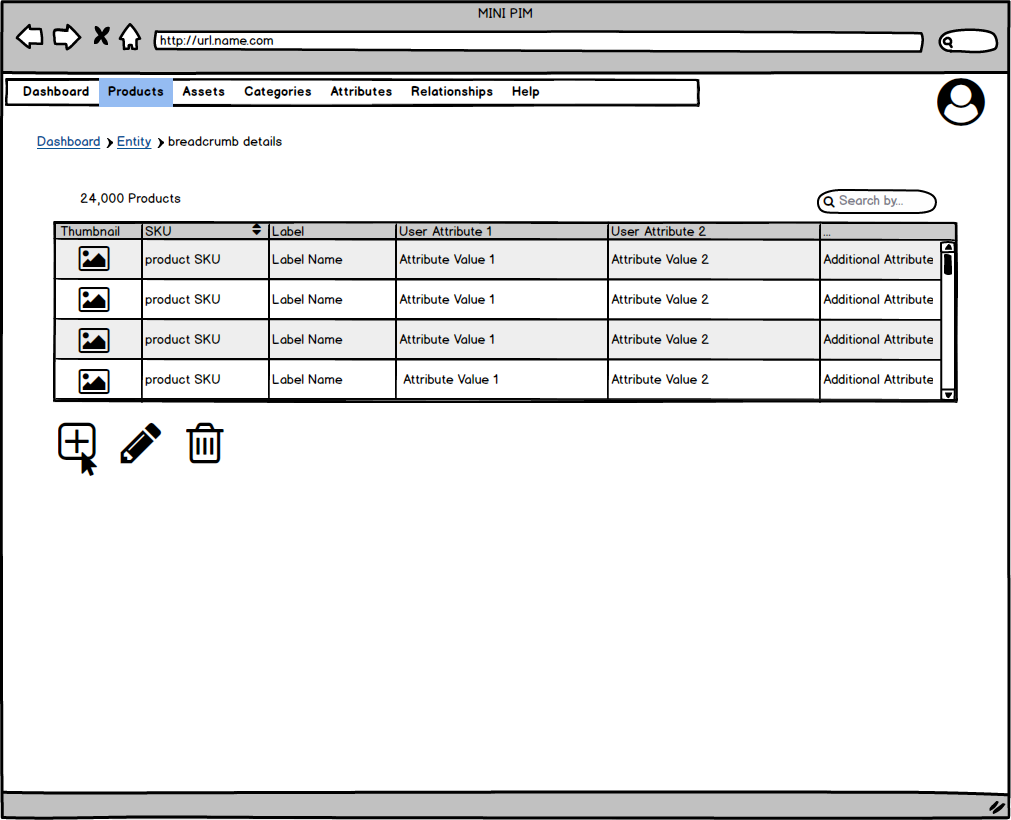
\includegraphics[width=1\linewidth]{mockups/RF2.1_boceto1.png}
    \caption{Apartado Productos hacer clic en \enquote{Añadir}}
   \end{figure}
\vspace{1.0cm}

\begin{figure}[H]
    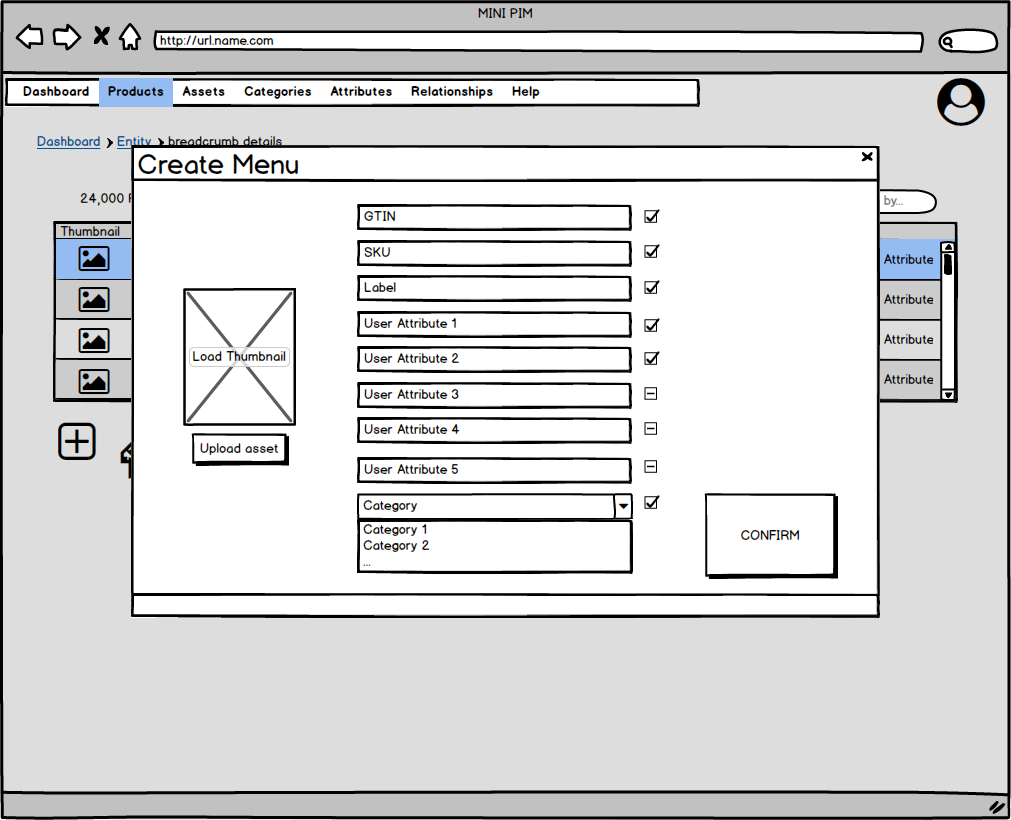
\includegraphics[width=1\linewidth]{mockups/RF2.1_bocetoCreacionV2.png}
    \caption{Menú de creación tras clicar \enquote{Añadir}}
   \end{figure}
\vspace{1.0cm}

\newpage %Inicia en una nueva página otro caso de uso